\chapter{Android}\label{sec:Android}
This chapter will provide information about Android and Wear 2.0 technology. Why it was developed and what are the differences between previous version and other wear technologies.

\medskip

Android is a Linux based operating system for mobile and wear devices developed by Google. The main selling point of this system is that it's open-source project, meaning everyone can access the code and modify it as they wish. Android was mainly developed for mobile phones but in time moved beyond and at this time is implemented into all kinds of wear devices, tablets, televisions and even refrigerators or cameras \cite{WIGA}.

\section{Android system structure}\label{sec:AndroidSystemStructure}
Android is created as a stack, meaning there are functional modules stack on top of each other from Linux core over native libraries to applications as shown in \fref{fig6}. Android maintains complete software stacks to enable device creators to run and modify Android for their specific hardware. To support these modifications and testing every release has multiple \enquote{code lines} to separate stable versions from experimental work \cite{AOSP}.

\begin{figure}[H]
	\begin{centering}
		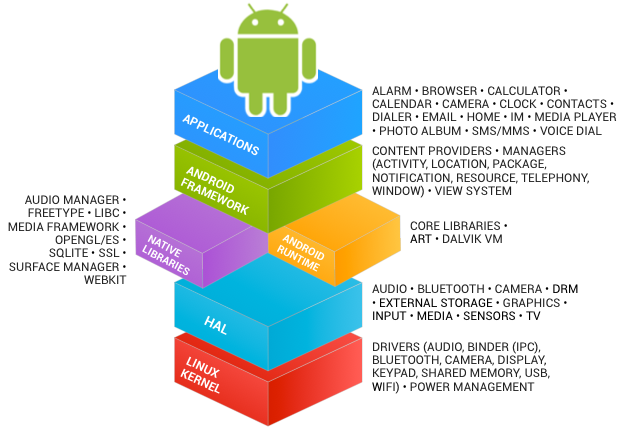
\includegraphics[width=0.6\textwidth]{img/android_stack}
		\par\end{centering}
	\caption{Android stack (source: \cite{AOSP})\label{fig:AndroidStack}}
	\label{fig6}
\end{figure}

There are multiple versions of Android system at this time and every single one has it's own version, code name and API level. Version codes are number identifications of a specific system version. Highest levels of these numbers are grouped into code names that are ordered alphabetically. As an example versions 8.0.0 and 8.1.0 have the same code name called Oreo. Finally API level is number identification for compatibility of specific application and it will be compared to API level of device Android system \cite{AOSP, AD}.

The highest part of the Android system stack are applications which extend device functionality and are written primarily in Java programming language \cite{SoASTaD}. These application are packaged into \verb|.apk| file, which is a zip archive, containing all application files like Java classes, layouts, images and more. The most important file is \verb|AndroidManifest.xml| that contains all meta-data about the application, such as permissions, package name, used components, versions and so forth. These application can be shared, for a nominal fee, via official market called Google Play. At the end of 2017 there were over three and a half million applications available in Google Play Store \cite{SoASTaD, NoAAiGPS, NoAA}.

Android is platform designed to be open source and free which makes it easy to create malicious applications. These application can bypass existing security and steal sensitive data, use telephony services or even gain control over the device \cite{ASIMPD}. Android has multiple ways to protect against such applications one of the most notable ones are Android Permission Framework and Google Play Protect \cite{SoASTaD}.

%T_ODO: describe Permissions and google play protect

\section{Wear technologies}\label{sec:WearTechnologies}
Interactive wearable, as an example smartwatches, is a new part of mobile computers. Wear devices are categorically different from phones or tables in term of usage, design and user interfaces (UI). According to the app design guidelines by major vendors, users interact with wearable devices frequently throughout daily use. Each interaction is short, often less than 10 seconds, and is dedicated to simple tasks \cite{UtCoAWO}. 

Important thing to note is that there are multiple kinds of wear devices from smart watches, wristbands, cameras or even glasses \cite{MIWD}. Based on report from Gartner technology research, conducted in 2017, most used wear devices were Bluetooth headset, wristbands and smartwatch \cite{GSWWDS}. Thanks to their small size wear devices are ideal to use for hands-free communication and health monitoring.

One problem with this diversity is hardware and software compatibility. Every device creator can create their own operating system for specific wear device and it can be difficult to develop custom applications for it. To avoid such problems this thesis is focused only on smartwatch with Android Wear operating system. 

There are three main points to note with watch devices. First, small battery capacity that can be almost ten times smaller then in typical smartphone. Second, point is display with around forty-times less pixels which completely changes properties. Final, scaled down CPU with high efficiency \cite{UtCoAWO}. Last two points are main parts of lowering power consumption of smartwatches but even with these cuts high-end watch devices can have really small battery life only in matter of few days or just hours.

\subsection{Android Wear}\label{sec:AndroidWear}
Android Wear is a version of Android OS tailored to small-screen wearable devices. There are not too many changes from system for smartphone but one of the main differences can be seen in UI since system had to be adjusted for watch size \cite{CSUITW}. Due to scaled down processing power of watches Android Wear wirelessly offloads data to the smartphone for heavy computing tasks, e.g., voice recognition \cite{UCAW}.

\begin{figure}[H]
	\begin{centering}
		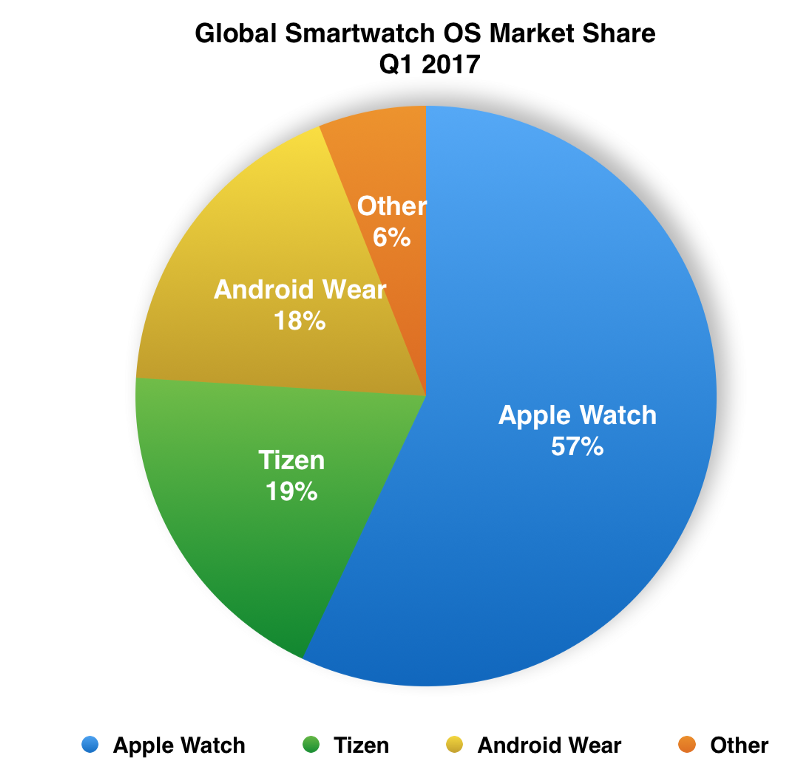
\includegraphics[width=0.6\textwidth]{img/wear_market_share}
		\par\end{centering}
	\caption{Smartwatch OS market share (source: \cite{TOAW})\label{fig:SmartwatchOSMarketShare}}
	\label{fig7}
\end{figure}

Android Wear is one of the most popular smartwatch systems but comes with it is own set of problems. Most notable and annoying one is being unable to pair wear with specific mobile device. It can be caused by combination of things such as system compatibility, custom hardware or phone type but it is more common then it should be \cite{AWPaS}. Having phone connected to Android Wear can also cause phone to drain battery way faster. One thing to note is that smartwatch can be connected to only single device and connecting to another requires factory reset. Few other problems can be update issues, notifications not coming through to the watch, not being able to connect to Wi-Fi and system crashes \cite{WAWP}.

Even with all these problems it is popular system and in early 2017 it got it's biggest update yet. New version 2.0 brought numerous improvements and features and few of the most notable ones will be described in this section \cite{AW2UG, AW2WN, AW2N}.

\subsubsection{Standalone applications}\label{sec:StandaloneApplications}
This feature is crucial change and it means that watch applications do not need mobile phone to function. Before this version it was needed to have connected phone with Android Wear support to use applications. Being forced to have Android phone proved as an obstacle for users without one since they could not use any applications on the watch \cite{AW2UG, AW2WN}.

Since application can now work without phone there should be a way to install them directly. Thankfully part of this update is also standalone Google Play Store where users can browse apps that are designed specifically for the watch \cite{AW2WN}. Part of this feature is also enabling watch to use wireless and cellular networks on their own since most standalone applications require this feature. And final part of this update was improving and securing communication with phone. This is now done via Wearable Data Layer API that is used in almost all Google applications and it is also pretty easy to use as a developer \cite{AW2UG}. 

\subsubsection{UI improvements}\label{sec:UIImprovements}
Part of new Android Wear version is implementation of Android's Material design guidelines \cite{DoAW}. It has much more \enquote{mature} look and darker design for reducing battery drain \cite{AW2WN}. It is completely focused on Wear devices and supports both round and square screens with new re-design of application launcher \cite{AW2UG}.

\begin{figure}[H]
	\begin{centering}
		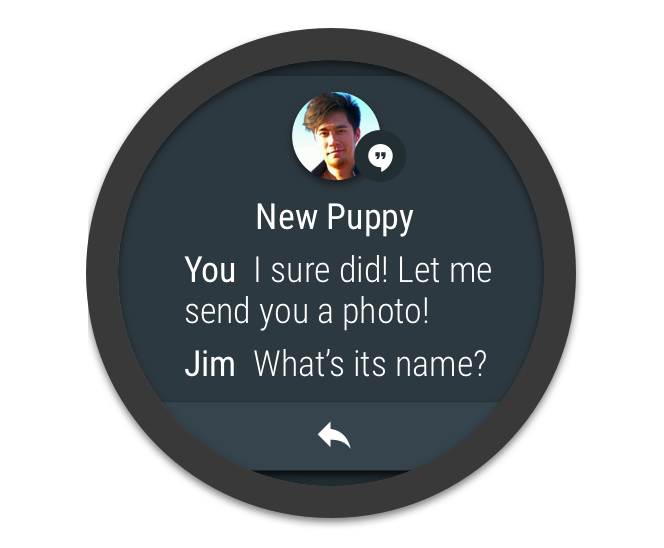
\includegraphics[width=0.3\textwidth]{img/wear_design_notification}
		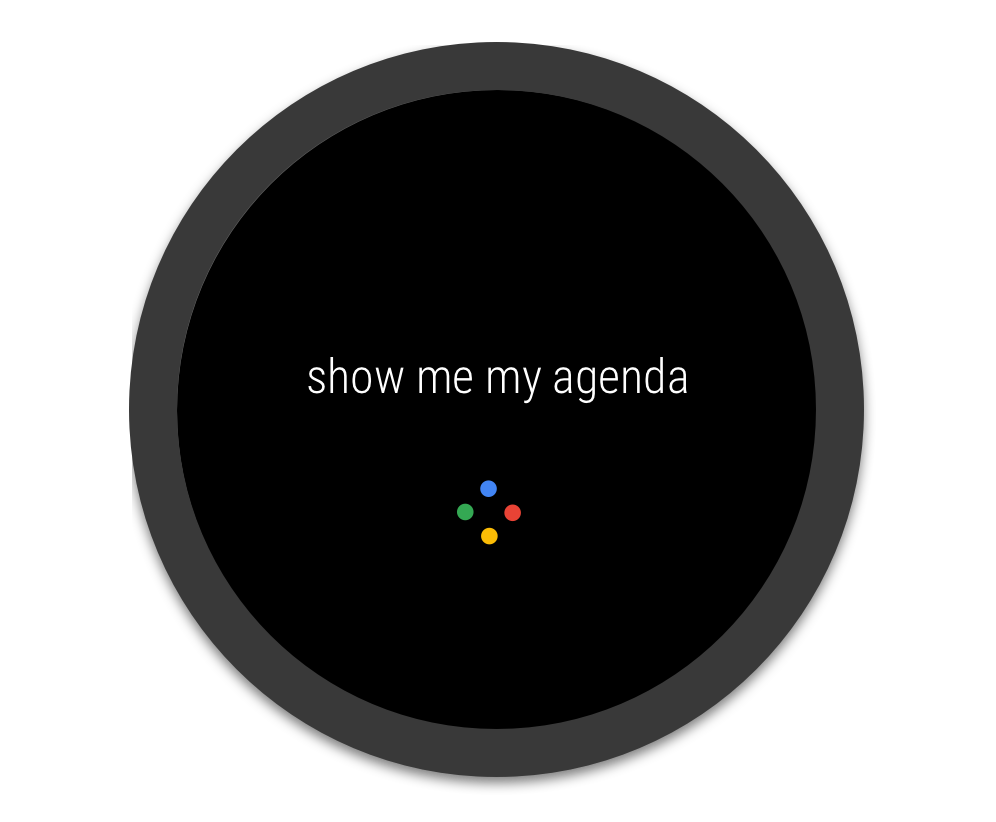
\includegraphics[width=0.3\textwidth]{img/wear_design_agenda}
		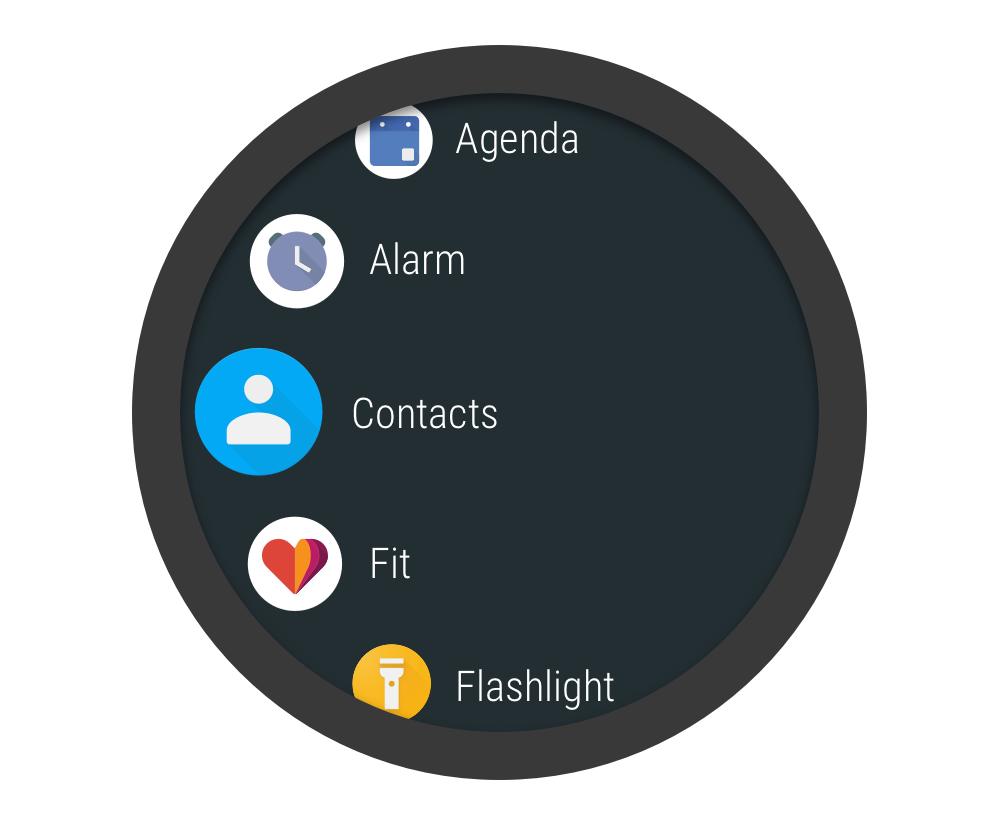
\includegraphics[width=0.3\textwidth]{img/wear_design_menu}
		\par\end{centering}
	\caption{Wear design examples (source: \cite{DoAW})\label{fig:WearDesignExamples}}
	\label{fig8}
\end{figure}

Android is also trying to catch up with Apple's watchOS and make default watch display, also called watch faces, much more useful. Users can add different widgets of any containing data of any application to the watch faces \cite{AW2UG}. This ensures quick access to the data user deems important \cite{AW2N}. All this data displays also match design of currently selected watch face and after clicking it will direct right into the application \cite{AW2WN}.

\begin{figure}[H]
	\begin{centering}
		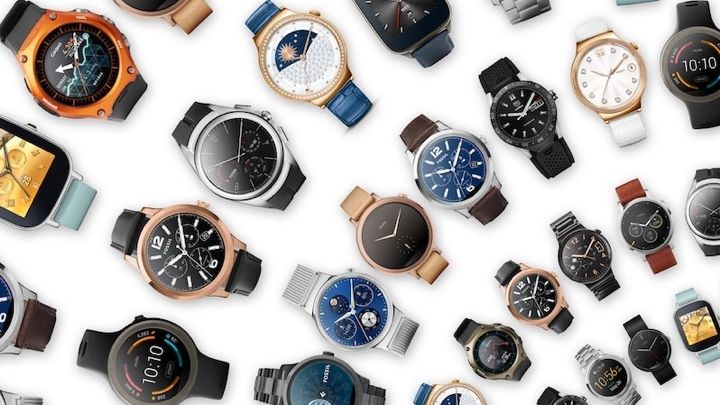
\includegraphics[width=0.5\textwidth]{img/wear_watch_faces}
		\par\end{centering}
	\caption{Wear watch faces (source: \cite{AW2UG})\label{fig:WearWatchFaces}}
	\label{fig9}
\end{figure}

\subsubsection{Google Assistant}\label{sec:GoogleAssistant}
Google Assistant is basically voice controlled smart assistant same as for example Amazon's Alexa, Apple's Siri or Microsoft's Cortana. There are multiple tech sites that run benchmarks of these systems \cite{ASGA, VACCGASAB, CAGACS, GASBAC} and they do not seem to be that different so there is no need to buy one over the other. These systems can pull information that you need or want and they track where you work, sports you like, your schedule, stuff that might interest you and much more \cite{WIGA}. With the update of Wear 2.0 this feature is now available on smartwatches \cite{AW2UG, AW2WN}.

\section{Other wear technologies}\label{sec:OtherWearTechnologies}
Tizen, Pebble, Apple, ...